\subsection{Experiment Interfaces}

\subsubsection{Mechanical Interfaces}
\label{sec:4.2.1}

\bigskip
\begin{table}[H]
\noindent\makebox[\columnwidth]{%
\scalebox{0.8}{
\begin{tabular}{|c|c|c|c|c|c|}
\hline
\textbf{Component} & \textbf{Interface} & \textbf{Amount} & \textbf{Dimensions} &  \begin{tabular}[c]{@{}c@{}}\textbf{Total}\\ \textbf{weight}\end{tabular}  \\ \hline
Bracket standard 20/20 slot 6/6 & AAC-Gondola & $8$ & $20 \times 20 \times 20\ mm$ & $40\ g$ \\ \hline
Tolerance holes bracket & CAC-Gondola & $2$ & $ 20 \times 30 \times 52 \ mm$ & $50\ g$ \\ \hline
4-hole plate & AAC-CAC & $6$ & $1 \times 60 \times 45\ mm$ & $100\ g$ \\ \hline
Rubber bumpers M6 & AAC-Gondola, CAC-Gondola & $10$ & $19 \times 19 \times 15\ mm$ & $300\ g$ \\ \hline
T-nut slot 6 M4 & AAC-CAC, AAC-Gondola, CAC-Gondola & $44$ & $4 \times 5.9 \times 11.5\ mm$ & $132\ g$ \\ \hline
T-nut slot 8 M6 & AAC-Gondola, CAC-Gondola & $10$ & $6 \times 11 \times 16\ mm$ &  $60\ g$ \\ \hline

Steel bolt M4 & AAC-CAC, AAC-Gondola & $44$ & $8\ mm $ length & $34\ g$ \\ \hline
Steel washer M4 & AAC-CAC, AAC-Gondola & $24$ &\begin{tabular}[c]{@{}c@{}}$ID=4.3\ mm$\\ $OD=9\ mm$\end{tabular} &  $4.8\ g$\\ \hline
% Polyamide bolt M4 & Styrofoam-CAC-AAC & $8$ & $20\ mm $ length & $3\ g$ & $24\ g$ \\ \hline
% Polyamide washer M4 & Styrofoam-CAC-AAC & $8$ &\begin{tabular}[c]{@{}c@{}}$ID=4.3\ mm$\\ $OD=25\ mm$\end{tabular} & $4\ g$ & $32\ g$\\ \hline
Styrofoam bars  & AAC-Gondola, CAC-Gondola & $4$ & see Appendix \ref{sec:mech_drawings} & $450\ g$ \\ \hline
Handles  & CAC \& AAC & $4$ & $ 18.6 \times 25.2 \times 112.5 \ mm$ & $80\ g$ \\ \hline
\end{tabular}}}
\caption{Summary of Gondola-AAC-CAC Interfaces Components.}
\label{table:attaching-components}
\end{table}


\underline{Gondola - TUBULAR joining}

\smallskip
The experiment box will be fixed to the gondola rails by means of $10$ brackets interfacing the experiment outside structure with the hammer nuts in the rails. Two different types of brackets are used to be flexible with respect to the gondola rails distances, which can be modified by use after previous BEXUS campaigns. Eight small $20/20$ brackets (Figure \ref{fig:bracket_small}) are used to fix the AAC box to specific rails placement, and two other big brackets (Figure \ref{fig:bracket_big}) are used to fix the CAC box to the nearest rail. This method is secure as well as fast enough to provide an accessible and easy recovery for later analysis.

\begin{figure}[H]
    \noindent\makebox[\textwidth]{%
    \begin{subfigure}{.3\textwidth}
        \centering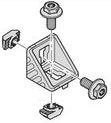
\includegraphics[width=0.55\textwidth]{4-experiment-design/img/Mechanical/bracket.jpg}
        \caption{Rexroth 20/20.}
        \label{fig:bracket_small}
    \end{subfigure}
    \hspace{1cm}
    \begin{subfigure}{.3\textwidth}
        \centering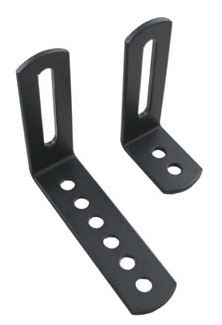
\includegraphics[width=0.55\textwidth,angle=90] {4-experiment-design/img/Mechanical/long_hole_bracket.jpg}
        \caption{Tolerance Holes.}
        \label{fig:bracket_big}
    \end{subfigure}}
    \caption{Bracket Components.}
    \label{fig:bracket}
\end{figure}

\bigskip
\underline{CAC - AAC joining}

\smallskip
A simple but reliable fixing interface between the two boxes of the experiment has been designed to ensure the fast recovery of the CAC box. The latter requires only unscrewing 12 bolts as well as unplugging a D-Sub connector marked in RED, see Figure \ref{fig:electrical_interfaces}. Once the CAC box is detached, the AAC Box will still remain perfectly fixed in the gondola. Table \ref{table:attaching-components} includes all the components required to fix the experiment to the gondola.

\bigskip
\underline{Handles}

\smallskip
Four top handles, as shown in Figure \ref{fig:handles} will be mounted to facilitate the experiment box manipulation when moving it in and out of the gondola.

\begin{figure}[H]
    \centering
    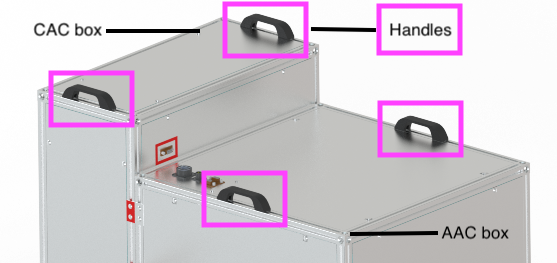
\includegraphics[width=0.8\textwidth]{4-experiment-design/img/Mechanical/Figure_8.png}
    \caption{Handling Interfaces.}
    \label{fig:handles}
\end{figure}

\bigskip
\underline{Inlet/Outlet Pipes}
\label{subsec:pipes}

\smallskip
In order to collect reliable air samples, the experiment requires to be mounted with at least one side exposed to the outside. This will reduce the pipe length used to collect clean air. As it can be seen in Figure \ref{fig:3D_tubular_render}, three pipes will extend from the experiment box face: one for the CAC sampling and two, input and output, for the AAC sampling. 

These pipes are welded/drawn $304$ grade stainless steel tubes from RESTEK company, which are specially recommended for chromatography applications and gas delivery systems with low pressures and inert environments. These tubes are sulfinert, which is a required treatment for metal components when analyzing for parts-per-billion levels of organo-sulfur compounds.

The tubes, which are the same that will be used in the pneumatic system of the \emph{Brain} (see Section \ref{sec:4.4.5}), have an outer diameter $OD = 6.35\ mm$ ($1/4$ inches) and an inner diameter $ID = 4.57\ mm$ ($0.18$ inches).

\bigskip
\underline{Pump vibration}
\label{subsec:vibration}

To mitigate the vibrations produced by the pump, an extra piece of styrofoam has been added between the pump's anchor plate and the surface of the level 1 of the brain, where this key component is fixed. 


\subsubsection{Thermal Interfaces}
\label{sec:4.2.2}

Both main structural components and external walls of the two boxes of the experiment are made by aluminum and steel components. For this reason, since these are conductive materials, a direct attachment to the gondola creates many heat paths with the internal space and subsystems of the experiment. Considering that the temperature gradient between the gondola and the operative requirements of the electronic components can be quite high, this conductive connections drastically decrease the efficiency of the thermal insulation. Therefore, a system based on rubber bumpers and styrofoam bars (see Figure \ref{fig:thermal_interface}) has been designed to remove heat bridges and minimize temperature leaks from the inside of the experiment to the outside.

Figure \ref{fig:rubber_bumper} shows a CAD model of the bumper component and how it looks like when attached to the gondola with the brackets explained in the previous section.

\begin{figure}[H]
    \noindent\makebox[\textwidth]{%
    \begin{subfigure}{.3\textwidth}
        \centering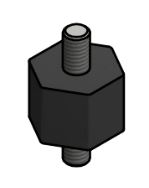
\includegraphics[width=0.55\textwidth]{4-experiment-design/img/Mechanical/rubber_bumper.jpg}
    \end{subfigure}
    \hspace{1cm}
    \begin{subfigure}{.3\textwidth}
        \centering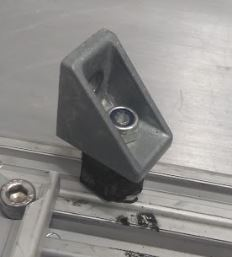
\includegraphics[width=0.55\textwidth] {4-experiment-design/img/Mechanical/real_bumper.jpg}
    \end{subfigure}}
    \caption{Rubber Bumper.}
    \label{fig:rubber_bumper}
\end{figure}

The styrofoam bars will be attached directly to the rails of the experiment structure by M4 plastic screws and big washers.

\begin{figure}[H]
    \centering
    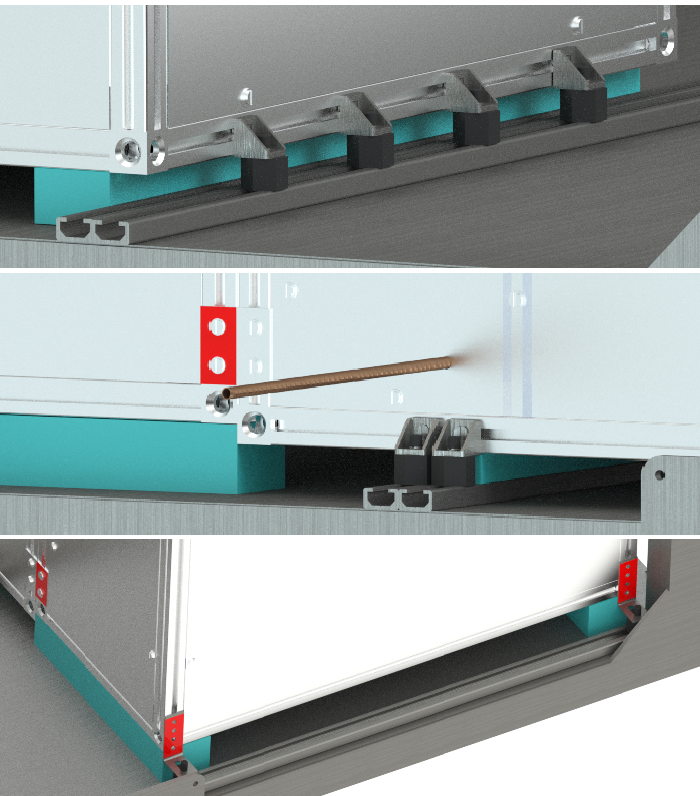
\includegraphics[width=0.6\textwidth]{4-experiment-design/img/Mechanical/gondola_fixation.png}
    \caption{Thermal Interfaces TUBULAR-Gondola.}
    \label{fig:thermal_interface}
\end{figure}

\subsubsection{CAC Interfaces}
An uncoupled quick connector, shown in Figure \ref{fig:Quick-connector-body}, will be attached at each end of the coiled tube to seal the opening. It will remain tightly sealed until the quick connectors are manually coupled. 

\begin{figure}[H]
    \centering
    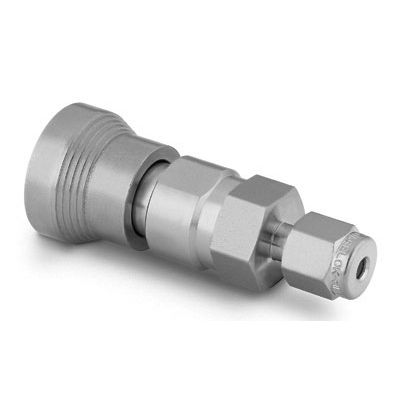
\includegraphics[width=0.2\textwidth]{4-experiment-design/img/Mechanical/CAC-QC-Outlet.jpg}
    \caption{Swagelok Quick Connector Body.}
    \label{fig:Quick-connector-body}
\end{figure}

The interfaces between the other parts in the CAC set up will be joined with specific tube fittings, listed in Table \ref{tab:CAC-interfaces}. All the chosen interfaces are from Swagelok. Using products from the same manufacture minimizes the risk for leakage or mismatched interfaces in the system. 

\begin{table}[H]
\centering
\scalebox{0.8}{
\begin{tabular}{|c|c|c|c|}
\hline
\textbf{Component}                                                          & \textbf{Interface}             & \textbf{Amount} & \textbf{Fitting Size}                                                    \\ \hline
\begin{tabular}[c]{@{}c@{}}Quick connector body\\ SS-QC4-B-200\end{tabular} & Outlet of coiled tube          & 1               & 1/8 in.                                                                  \\ \hline
\begin{tabular}[c]{@{}c@{}}Quick connector body\\ SS-QC4-B-400\end{tabular} & Inlet of coiled tube           & 1               & 1/4 in.                                                                  \\ \hline
\begin{tabular}[c]{@{}c@{}}Quick connector stem\\ SS-QC4-D-400\end{tabular} & Inlet of coiled tube -  Filter & 1               & 1/4 in.                                                                  \\ \hline
\begin{tabular}[c]{@{}c@{}}Male connector\\ SS-400-1-2\end{tabular}             & Tube fitting - Solenoid valve   & 2               & \begin{tabular}[c]{@{}c@{}}Tube OD 1/8 in. to \\ Tube OD 1/4 in.\end{tabular}    \\ \hline
\begin{tabular}[c]{@{}c@{}}Straight Tube Union\\ SS-200-6\end{tabular}             & Quick connector 1/8 in. - Tube 1/8 in.     & 1               & 1/8 in.
\\ \hline
\begin{tabular}[c]{@{}c@{}}Tube Reducer\\ SS-400-6-2 \end{tabular}             & Tube 1/8 in. - Tube 1/4 in.     & 1               & \begin{tabular}[c]{@{}c@{}}Tube OD 1/8 in. to \\ Tube OD 1/4 in.\end{tabular}
\\ \hline
\begin{tabular}[c]{@{}c@{}}Straight Tube Union\\ SS-400-6\end{tabular}             & Tube 1/4 in. - 90 degree connector    & 1               & 1/4 in.
\\ \hline
\begin{tabular}[c]{@{}c@{}}Union 90-degree connector\\ SS-400-9\end{tabular}             &
\begin{tabular}[c]{@{}c@{}} Between certain tube fittings\\ Outlet tube \end{tabular} & 3               & 1/4 in.
\\ \hline
\begin{tabular}[c]{@{}c@{}}Tube fitting\\ SS-401-PC\end{tabular}             & \begin{tabular}[c]{@{}c@{}} Between certain tube fittings\\ Magnesium dryer filter \end{tabular} & 5               & 1/4 in.
\\ \hline
\end{tabular}}
\caption{Interfaces within CAC Setup.}
\label{tab:CAC-interfaces}
\end{table}

\subsubsection{AAC Interfaces}
In the AAC system, the interfaces between various components are a mixture of eleven different types of tube fittings from Swagelok. The selected types are straight and elbow union, T-union, female and male elbows, male and female connectors, tube fittings, and quick coupling with a certain  specifications. Some of them are shown in Figure \ref{fig:AAC-interfaces-fittings}. Information regarding the fitting's placement in the AAC and fitting sizes are summarized in Table \ref{tab:AAC-interfaces}. 

\begin{figure}[H]
    \centering
    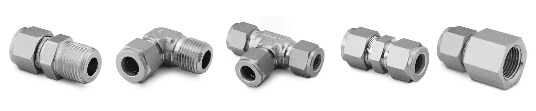
\includegraphics[width=0.8\textwidth]{4-experiment-design/img/Mechanical/AAC-interfaces.jpg}
    \caption{From Left to Right: Male Connector, Male Elbow, T-union, Straight Union and Female Connector.}
    \label{fig:AAC-interfaces-fittings}
\end{figure}

\begin{table}[H]
\centering
\scalebox{0.9}{
\begin{tabular}{|c|c|c|c|}
\hline
\textbf{Component}                                                    & \textbf{Interface}                                                                                                                                                                         & \textbf{Amount} & \textbf{Fitting Size}                                                                     \\ \hline
\begin{tabular}[c]{@{}c@{}}Male connector\\ SS-400-1-2\end{tabular}   & \begin{tabular}[c]{@{}c@{}}Airflow sensor - Sensor box\\ Tube sensor box - Manifold \\ Manifold - Flushing valve\\ Flushing valve - Outlet tube\\ Solenoid valve - Tube valve\end{tabular} & 11              & \begin{tabular}[c]{@{}c@{}}Male 1/8 in. to \\ Tube OD 1/4 in.\\ ID 0.21 in.\end{tabular}  \\ \hline
\begin{tabular}[c]{@{}c@{}}Male elbow\\ SS-400-2-2\end{tabular}       & Sensor box - Tube sensor box                                                                                                                                                               & 1               & \begin{tabular}[c]{@{}c@{}}Male 1/8 in. to \\ Tube OD 1/4 in.\\ ID 5/32 in.\end{tabular}  \\ \hline
\begin{tabular}[c]{@{}c@{}}Straight union\\ SS-400-6\end{tabular}     & \begin{tabular}[c]{@{}c@{}}Filter - Tube filter\\ Tube filter - Pump\\ Pump - Tube pump\end{tabular}                                                                                       & 3               & \begin{tabular}[c]{@{}c@{}}Tube OD 1/4 in.\\ ID 5/32 in.\end{tabular}                     \\ \hline
\begin{tabular}[c]{@{}c@{}}Female connector\\ SS-400-7-4\end{tabular} & \begin{tabular}[c]{@{}c@{}}Inlet tube - Filter\\ Tube pump - Airflow sensor\\ Airflow sensor - Tube airflow sensor\end{tabular}                                                            & 3               & \begin{tabular}[c]{@{}c@{}}Female 1/4 in. to\\ Tube OD 1/4 in.\\ ID 5/32 in.\end{tabular} \\ \hline
\begin{tabular}[c]{@{}c@{}}T-Union\\ SS-400-3\end{tabular}            & Tube valve - Bag valve                                                                                                                                                                     & 6               & Male 1/4 in.                                                                              \\ \hline
\end{tabular}}
\caption{Interface Descriptions Inside AAC System.}
\label{tab:AAC-interfaces}
\end{table}


\subsubsection{Electrical Interfaces}
\label{sec:4.2.3}

The experiment will connect to the gondola electrically via a 4 pin, male, box mount receptacle MIL - C-26482P series 1 connector with an 8-4 insert arrangement (MS3112E8-4P) \cite{BexusManual}. It will connect to one 28.8 V/1 mA battery pack which consists of eight SAFT LSH20 batteries in series where each has a 5 A fuse\cite{BexusManual}. The expected maximum current is 1.1 A.

\begin{figure}[H]
    \centering
    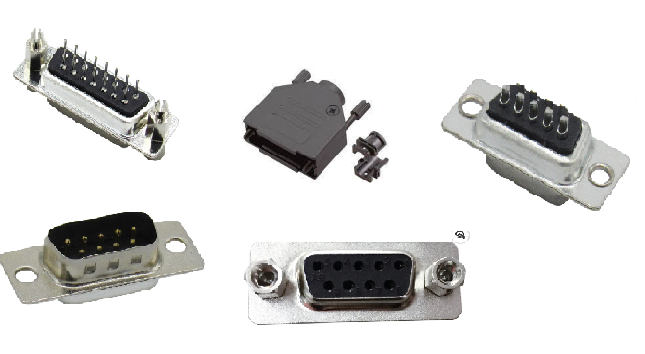
\includegraphics[width=0.4\textwidth]{4-experiment-design/img/connectors.png}
    \caption{Connectors.}
    \label{fig:connectors}
\end{figure}

The E-Link connection shall be made between the experiment and the E-Link system using a RJ45 connection which will be supplied by SSC and an Ethernet protocol. The Amphenol RJF21B connector will be mounted on either the front or the side of the experiment\cite{BexusManual}.  

The CAC and AAC will be connected together with a D-SUB 9-pin connector where power, ground and signals for the sensors in the CAC will be connected. A female connector will be located on the AAC wall and a male connector on the CAC wall.

Another female D-SUB 9-pin connector will be located on the wall of the AAC in which the connections for the three ambient pressure sensors will be located. Connectors with different pin configuration are shown in Figure \ref{fig:connectors}.

The expected data rate is 1.58 kbits/s for downlink and 1.08 kbits/s for uplink.

\begin{figure}[H]
    \centering
    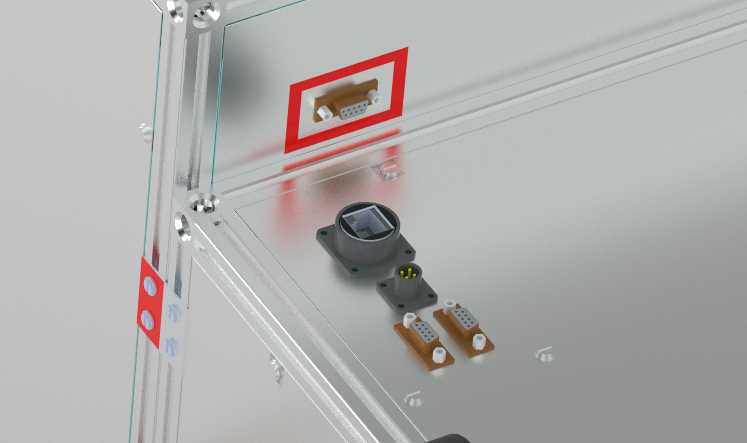
\includegraphics[width=0.8\textwidth]{4-experiment-design/img/Mechanical/Figure_Detail_Interfaces.png}
    \caption{Electrical Interfaces.}
    \label{fig:electrical_interfaces}
\end{figure}



%\begin{figure}[H]
%    \begin{align*}
%        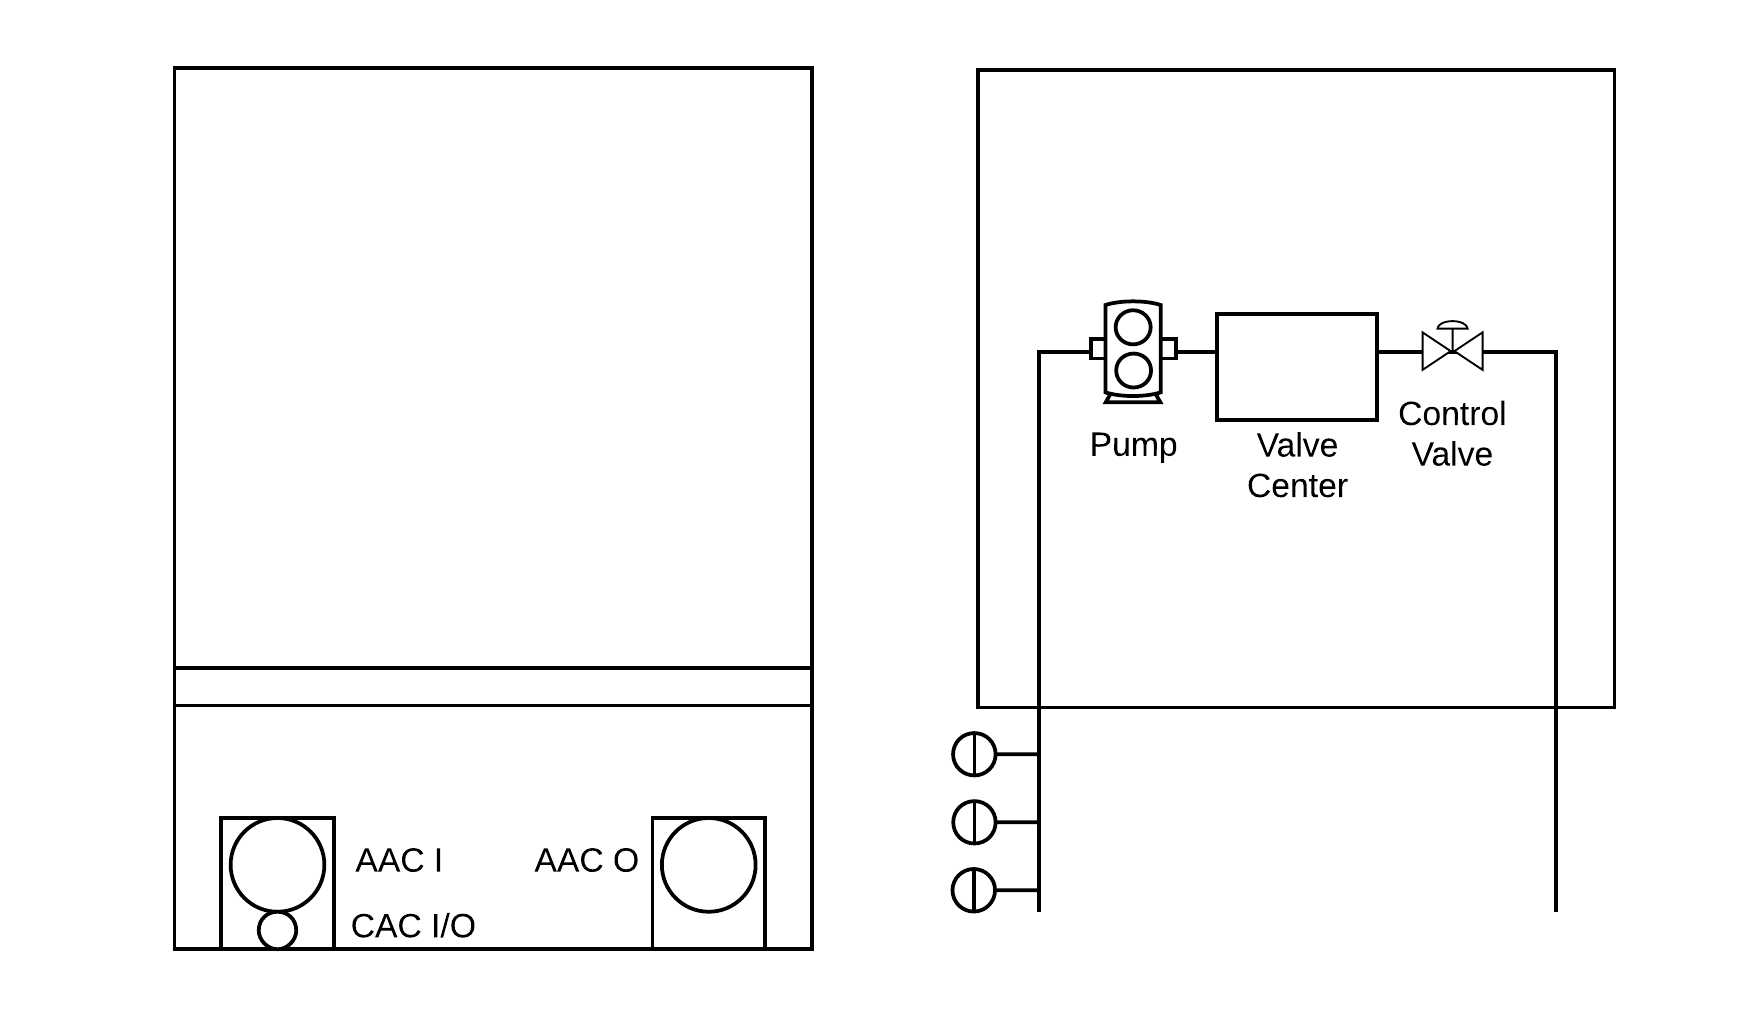
\includegraphics[width=0.7\textwidth]{4-experiment-design/img/Diagram_pipe.png}
%    \end{align*}
%    \caption{Diagram of the experiment box face exposed to the outside.}\label{fig:pipes_interface_1}
%\end{figure}

\iffalse
\subsubsection{Radio Frequencies (Optional)}
\begin{centering}
Not required.
\end{centering}
\bigskip

\subsubsection{Thermal (Optional)}
\begin{centering}
Not required.
\end{centering}
\bigskip
\fi


\raggedbottom